\documentclass{beamer}

\useoutertheme[subsection=false]{miniframes}
\usecolortheme{beaver}
\setbeamertemplate{navigation symbols}{}
\setbeamertemplate{footline}{}
\usepackage{graphicx}
\usepackage{url}
\usepackage{datetime}
\usepackage{tikz-cd}
\newcommand{\lectureDate}{\formatdate{22}{11}{2018}}

\setbeamertemplate{caption}
{\raggedright\insertcaption\par}
\title{MATH211: Linear Methods I}
\author{Matthew Burke}
\date{\lectureDate}
\begin{document}

\frame{\titlepage}

\begin{frame}{Lecture on \lectureDate}
  \tableofcontents
\end{frame}

\section*{Last time}
\label{sec:Last-time}

\begin{frame}{Last time}
	\begin{itemize}
		\item Converting to polar form.\vfill
		\item Converting from polar form.\vfill
		\item Multiplication using polar form.
	\end{itemize}
\end{frame}

\section{Examples}

\begin{frame}
\begin{beamercolorbox}[sep=12pt,center]{part title}
\usebeamerfont{section title}
\insertsection\par
\end{beamercolorbox}
\end{frame}

\begin{frame}{Examples}
\begin{example}
Express $(1-i)^6(\sqrt{3}+i)^3$ in the form $a+bi$. % ANS: -64
\end{example}
\begin{example}
Express $(\frac{1}{2}-\frac{\sqrt{3}}{2}i)^{17}$ in the form $a+bi$. % ANS: 1/2 + (sqrt{3}/2)i
\end{example}
\end{frame}

\section{Complex roots}

\begin{frame}
\begin{beamercolorbox}[sep=12pt,center]{part title}
\usebeamerfont{section title}
\insertsection\par
\end{beamercolorbox}
\end{frame}

\begin{frame}{Principal square roots}
Now we know that:\vfill
{\bf Slogan:} To multiply two complex numbers we multiply the moduli and add the angles.\vfill
So we could try reversing this:\vfill
{\bf Slogan:} To find the principal square root we take the square root of the modulus and halve the angle.\vfill
\begin{itemize}
	\item (The answer will depend on the angle measuring convention.)
\end{itemize}
\end{frame}

\begin{frame}{Picture}
If $z = e^{i\alpha}$ has unit modulus:\vfill
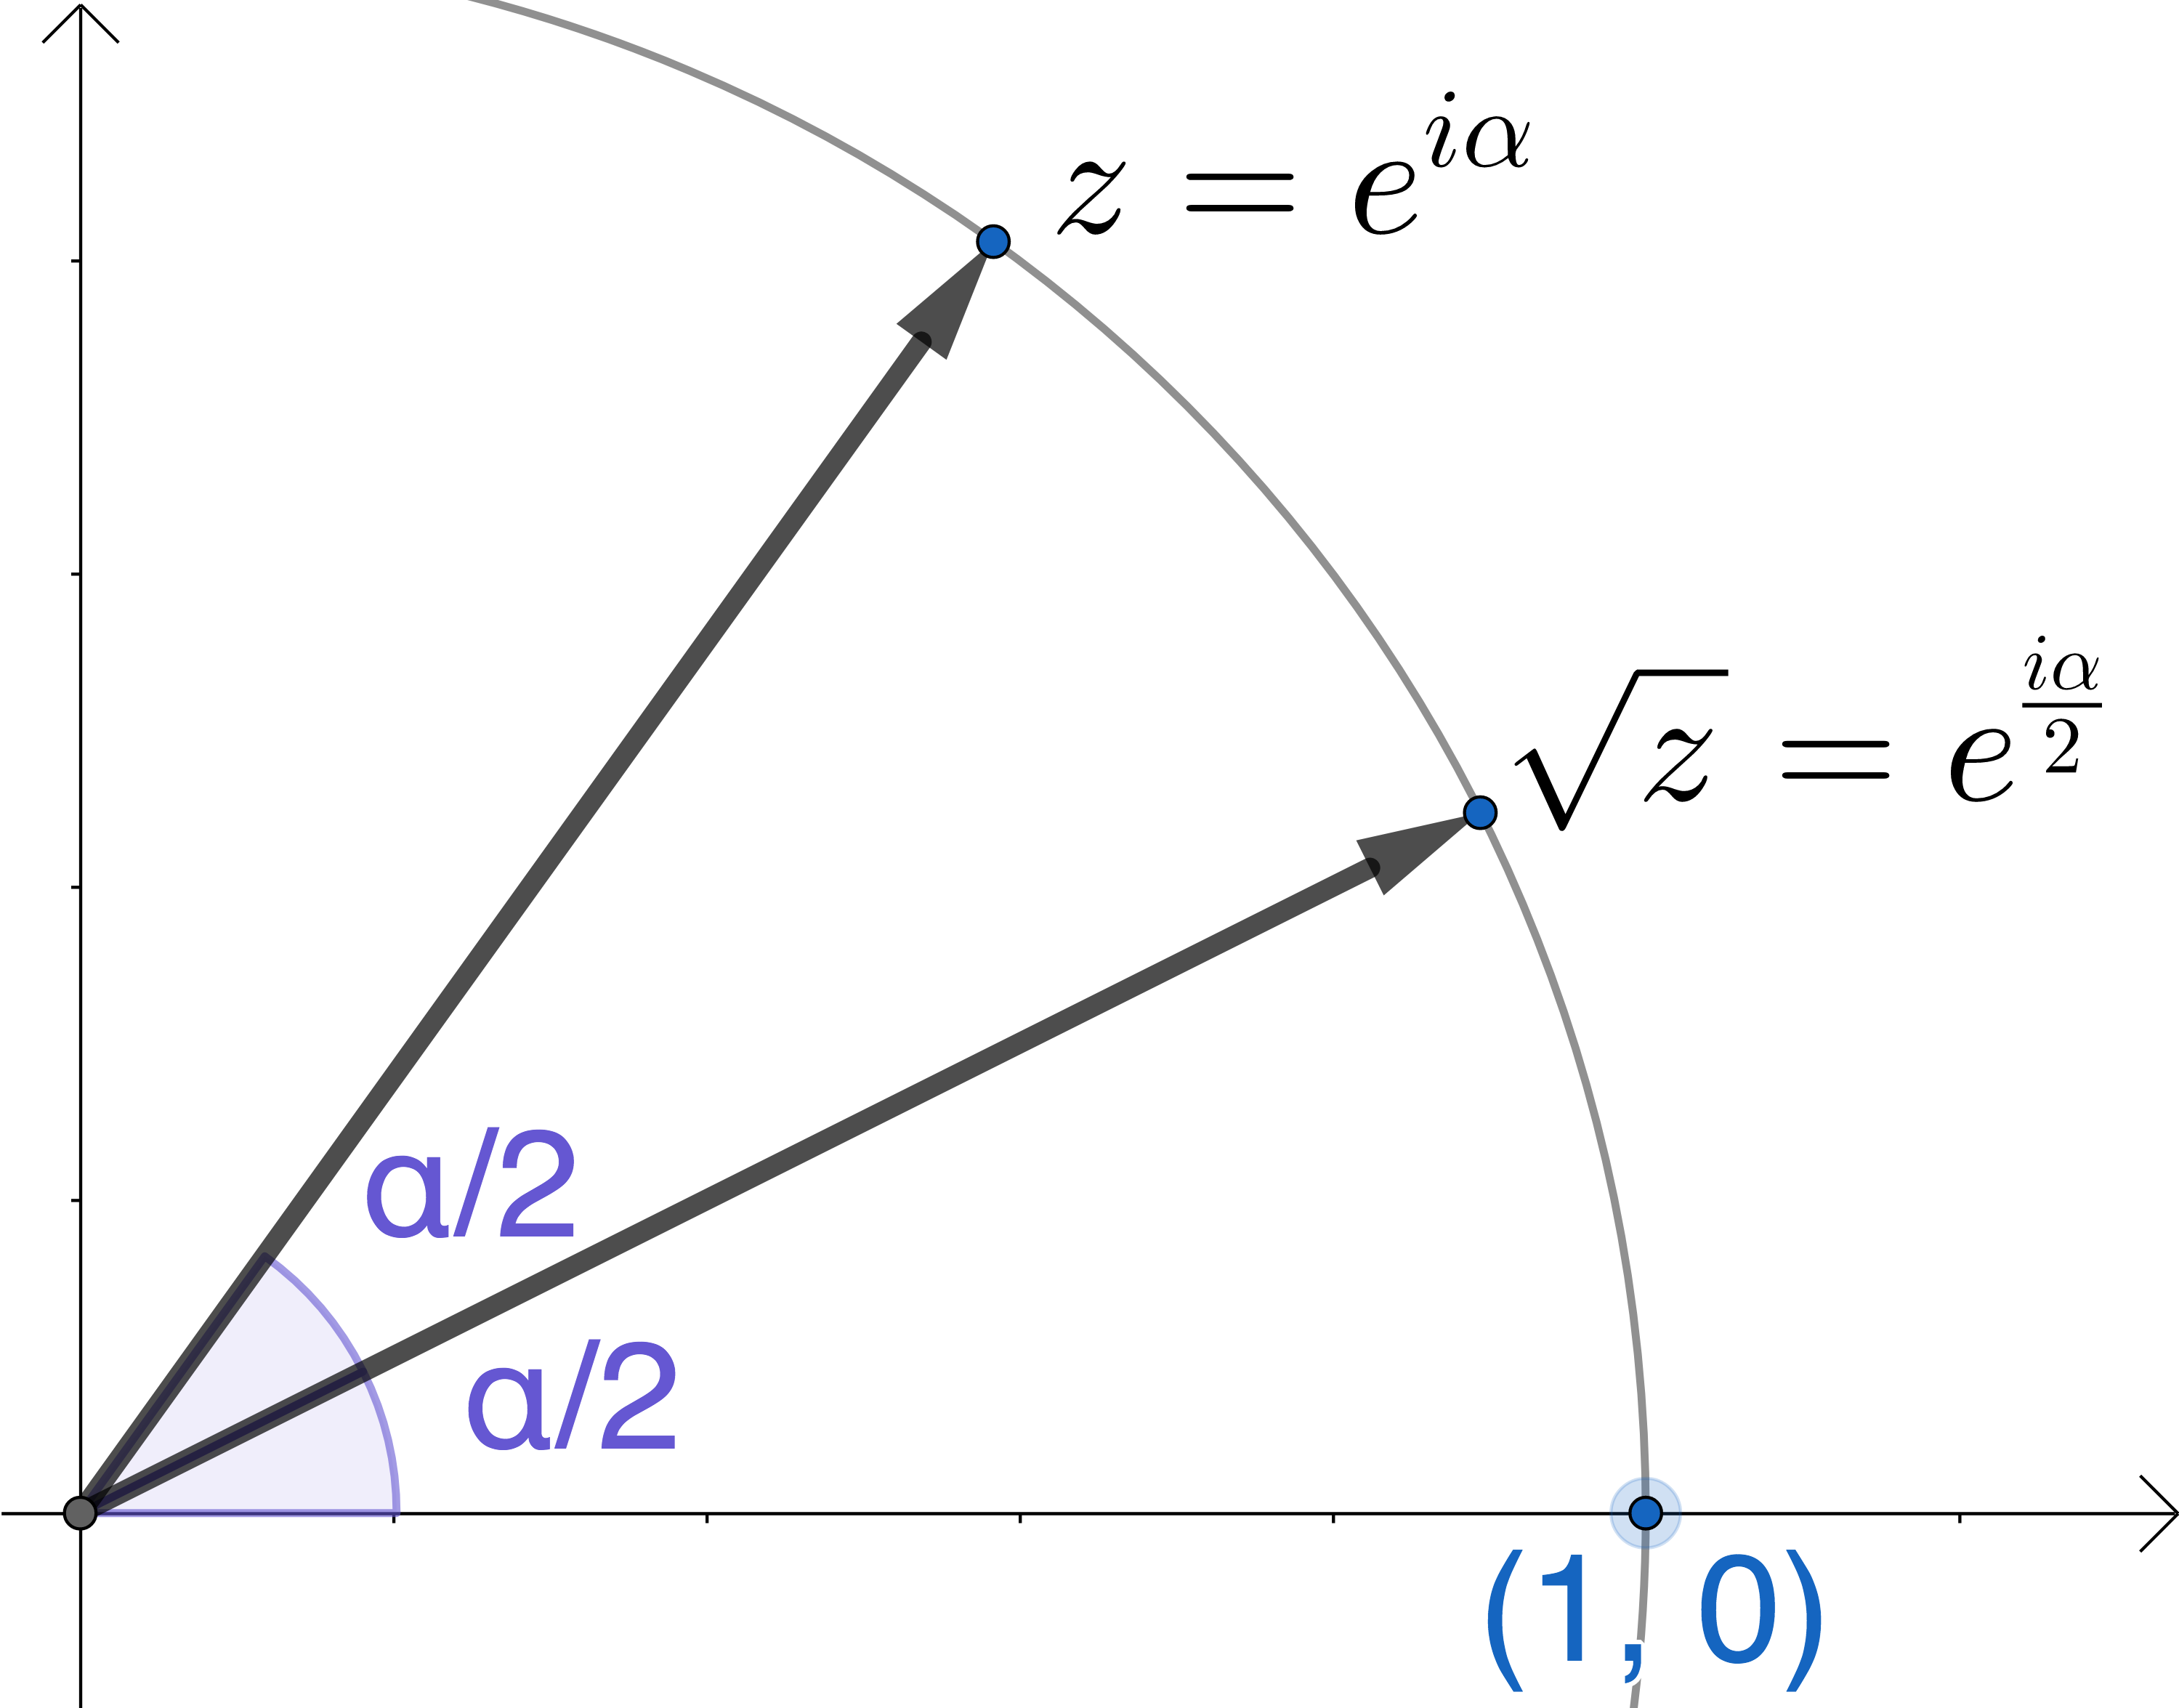
\includegraphics[scale=5]{principal-square-root.png}
\end{frame}

\begin{frame}{Non-principal square roots}
Let $z = R\cdot e^{i\alpha}$ and take the principal square root:\vfill
{\LARGE
\begin{equation*}
\sqrt{z} = \sqrt{R\cdot e^{i\alpha}} = \sqrt{R}\cdot e^{\frac{i\alpha}{2}}
\end{equation*}
}\vfill
Then all of numbers of the form\vfill
{\LARGE
\begin{equation*}
\sqrt{R}\cdot e^{(\frac{i\alpha}{2}+ki\cdot\pi)}
\end{equation*}
}\vfill
for $k\in \mathbb{Z}$ are \emph{also} a square roots of $z$:\vfill
{\LARGE
\begin{equation*}
\left(\sqrt{R}\cdot e^{(\frac{i\alpha}{2}+ki\pi)}\right)^2 = R\cdot e^{i\alpha + 2ki\pi} = R\cdot e^{i\alpha} = z
\end{equation*}
}
\end{frame}

\begin{frame}{Example}
  	The two square roots of $z = e^{\frac{i\pi}{4}}$ are $e^{\frac{i\pi}{8}}$ and $e^{\frac{-7i\pi}{8}}$:\vfill
	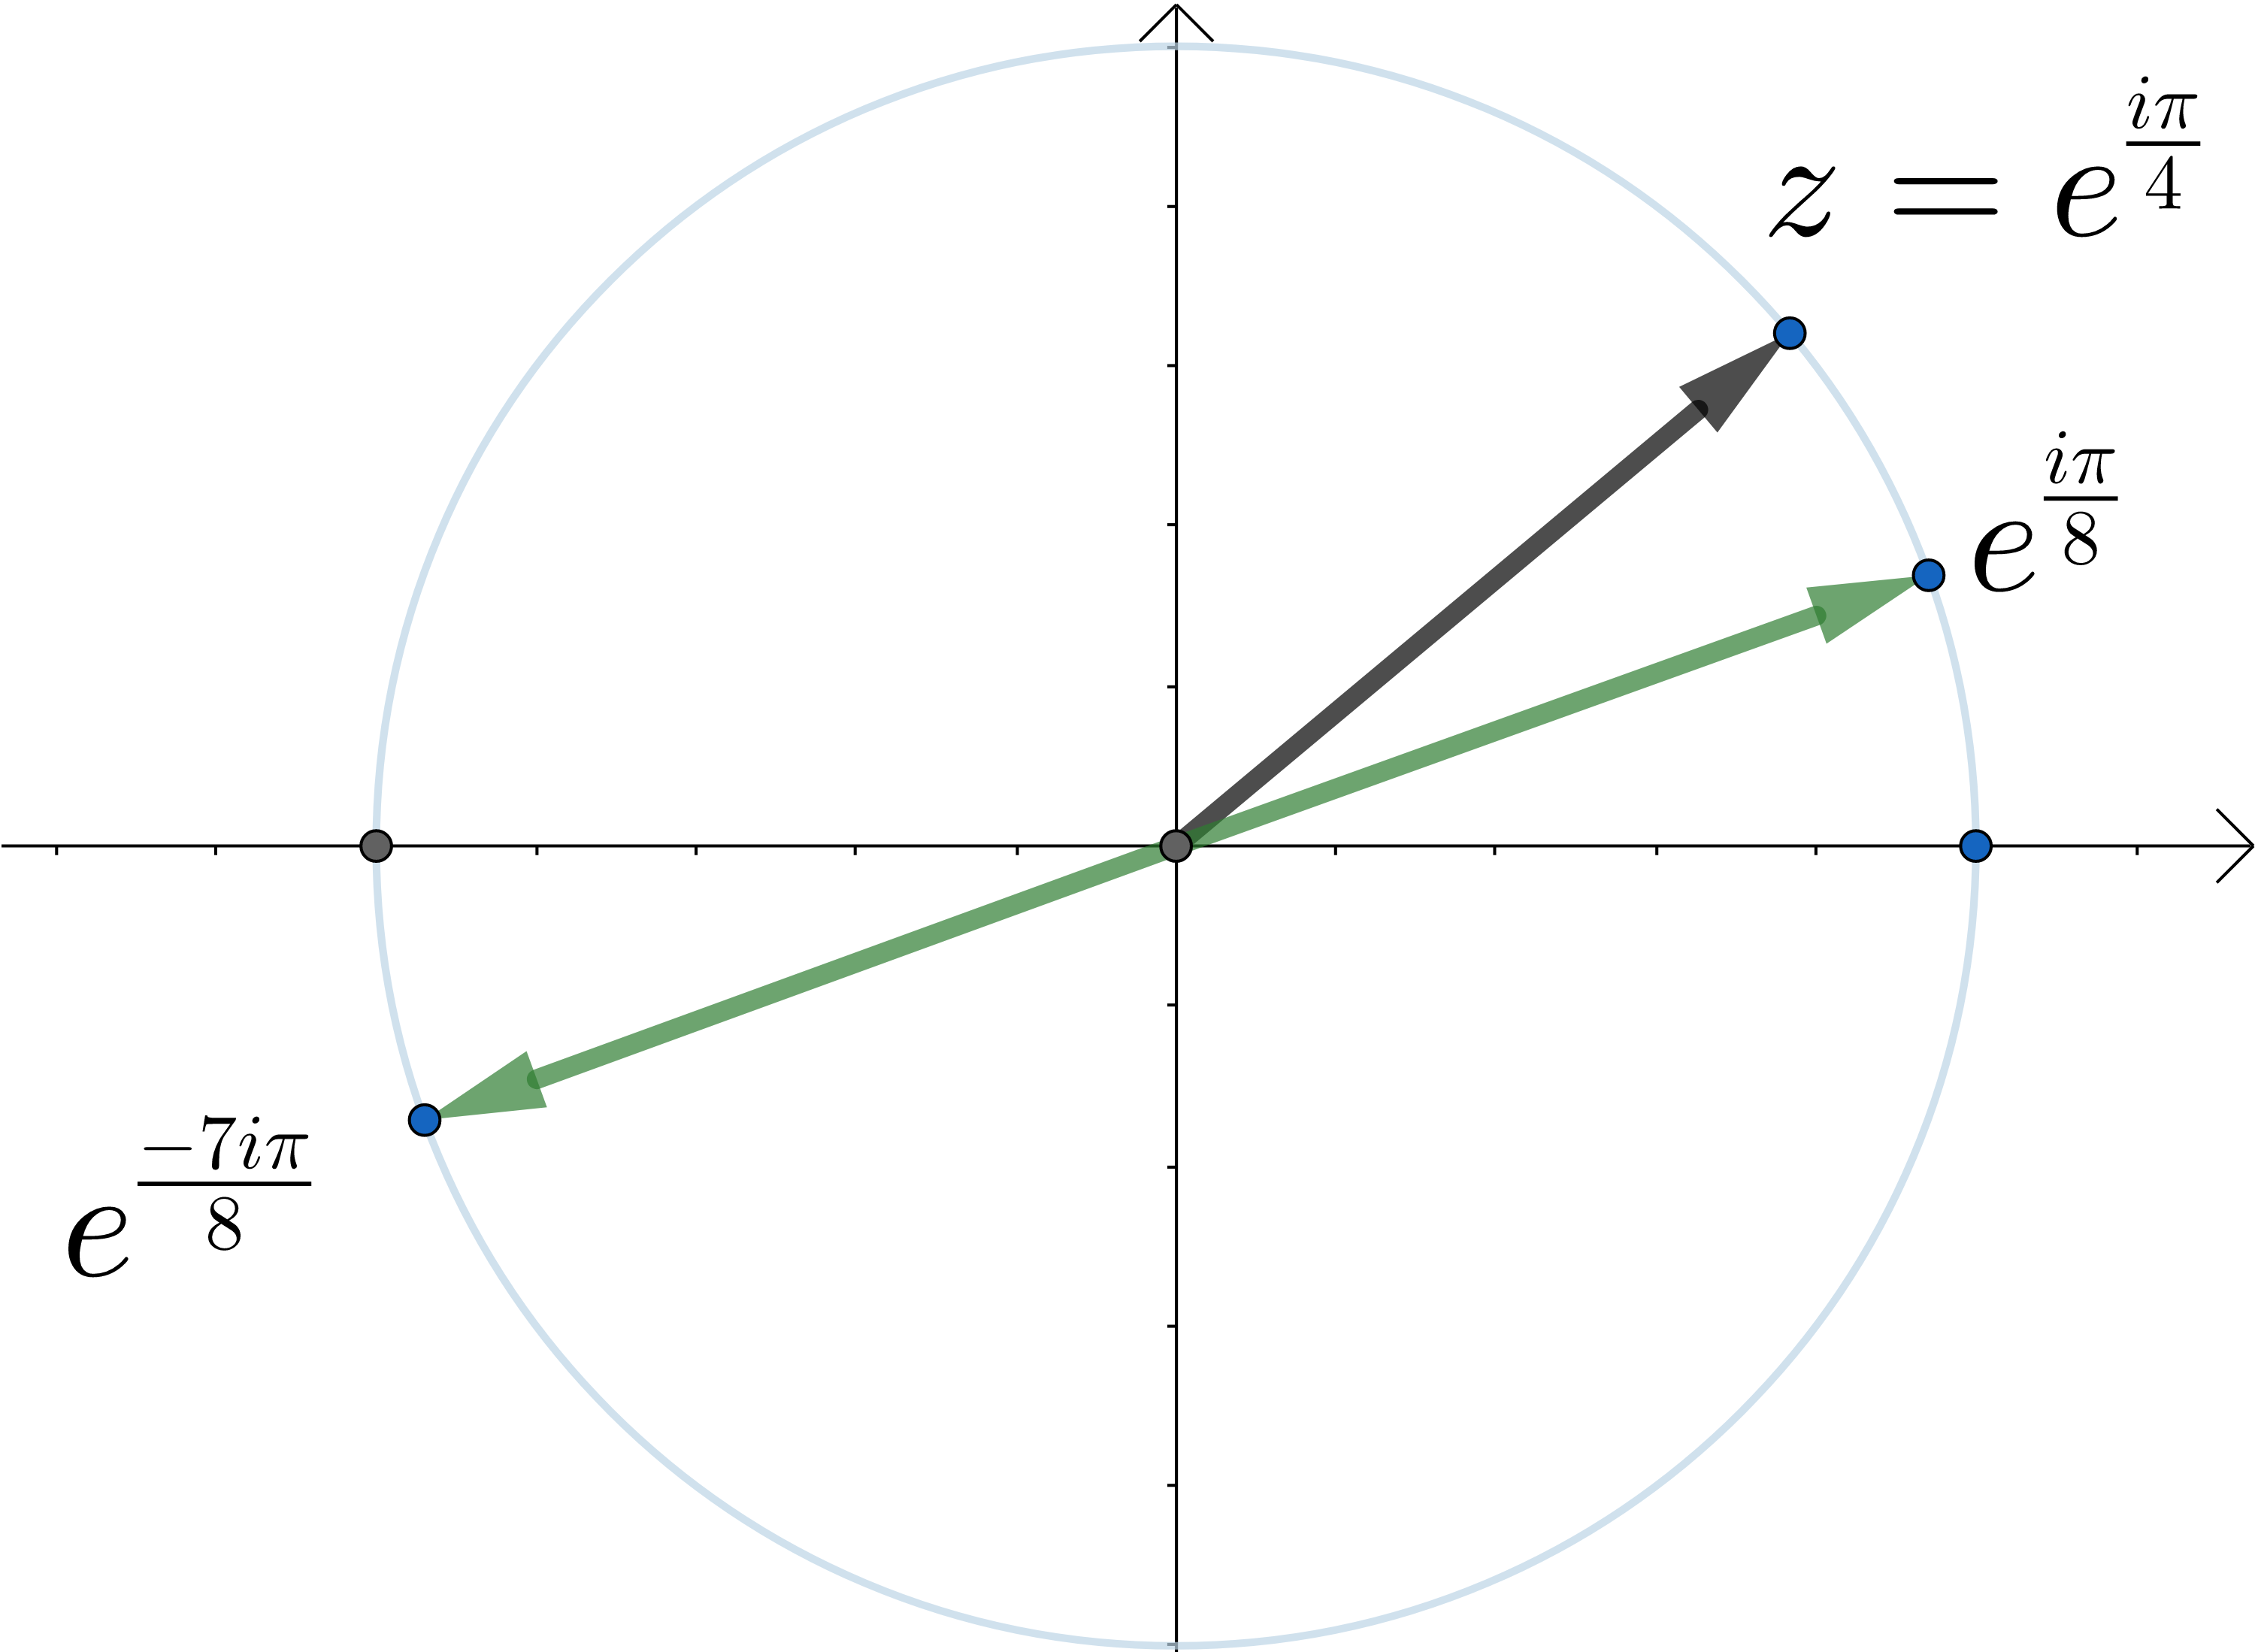
\includegraphics[scale=3]{roots-pi-4.png}
\end{frame}

\begin{frame}{N-th roots}
Similarly there is a principal $n$-th root:\vfill
{\LARGE
\begin{equation*}
\sqrt[n]{z} = \sqrt[n]{R\cdot e^{i\alpha}} = \sqrt[n]{R}\cdot e^{\frac{i\alpha}{n}}
\end{equation*}}\vfill
and all numbers of the form\vfill
{\LARGE
\begin{equation*}
	\sqrt[n]{R}e^{\frac{i\alpha+2ki\pi}{n}}
\end{equation*}
}\vfill
are also $n$-th roots of $z$ for $k\in \mathbb{N}$.
\end{frame}

\begin{frame}{Cube roots}
The cube roots of $8$ are $2$, $2e^{\frac{2i\pi}{3}}$ and $2e^{\frac{-2i\pi}{3}}$:\vfill
\begin{center}
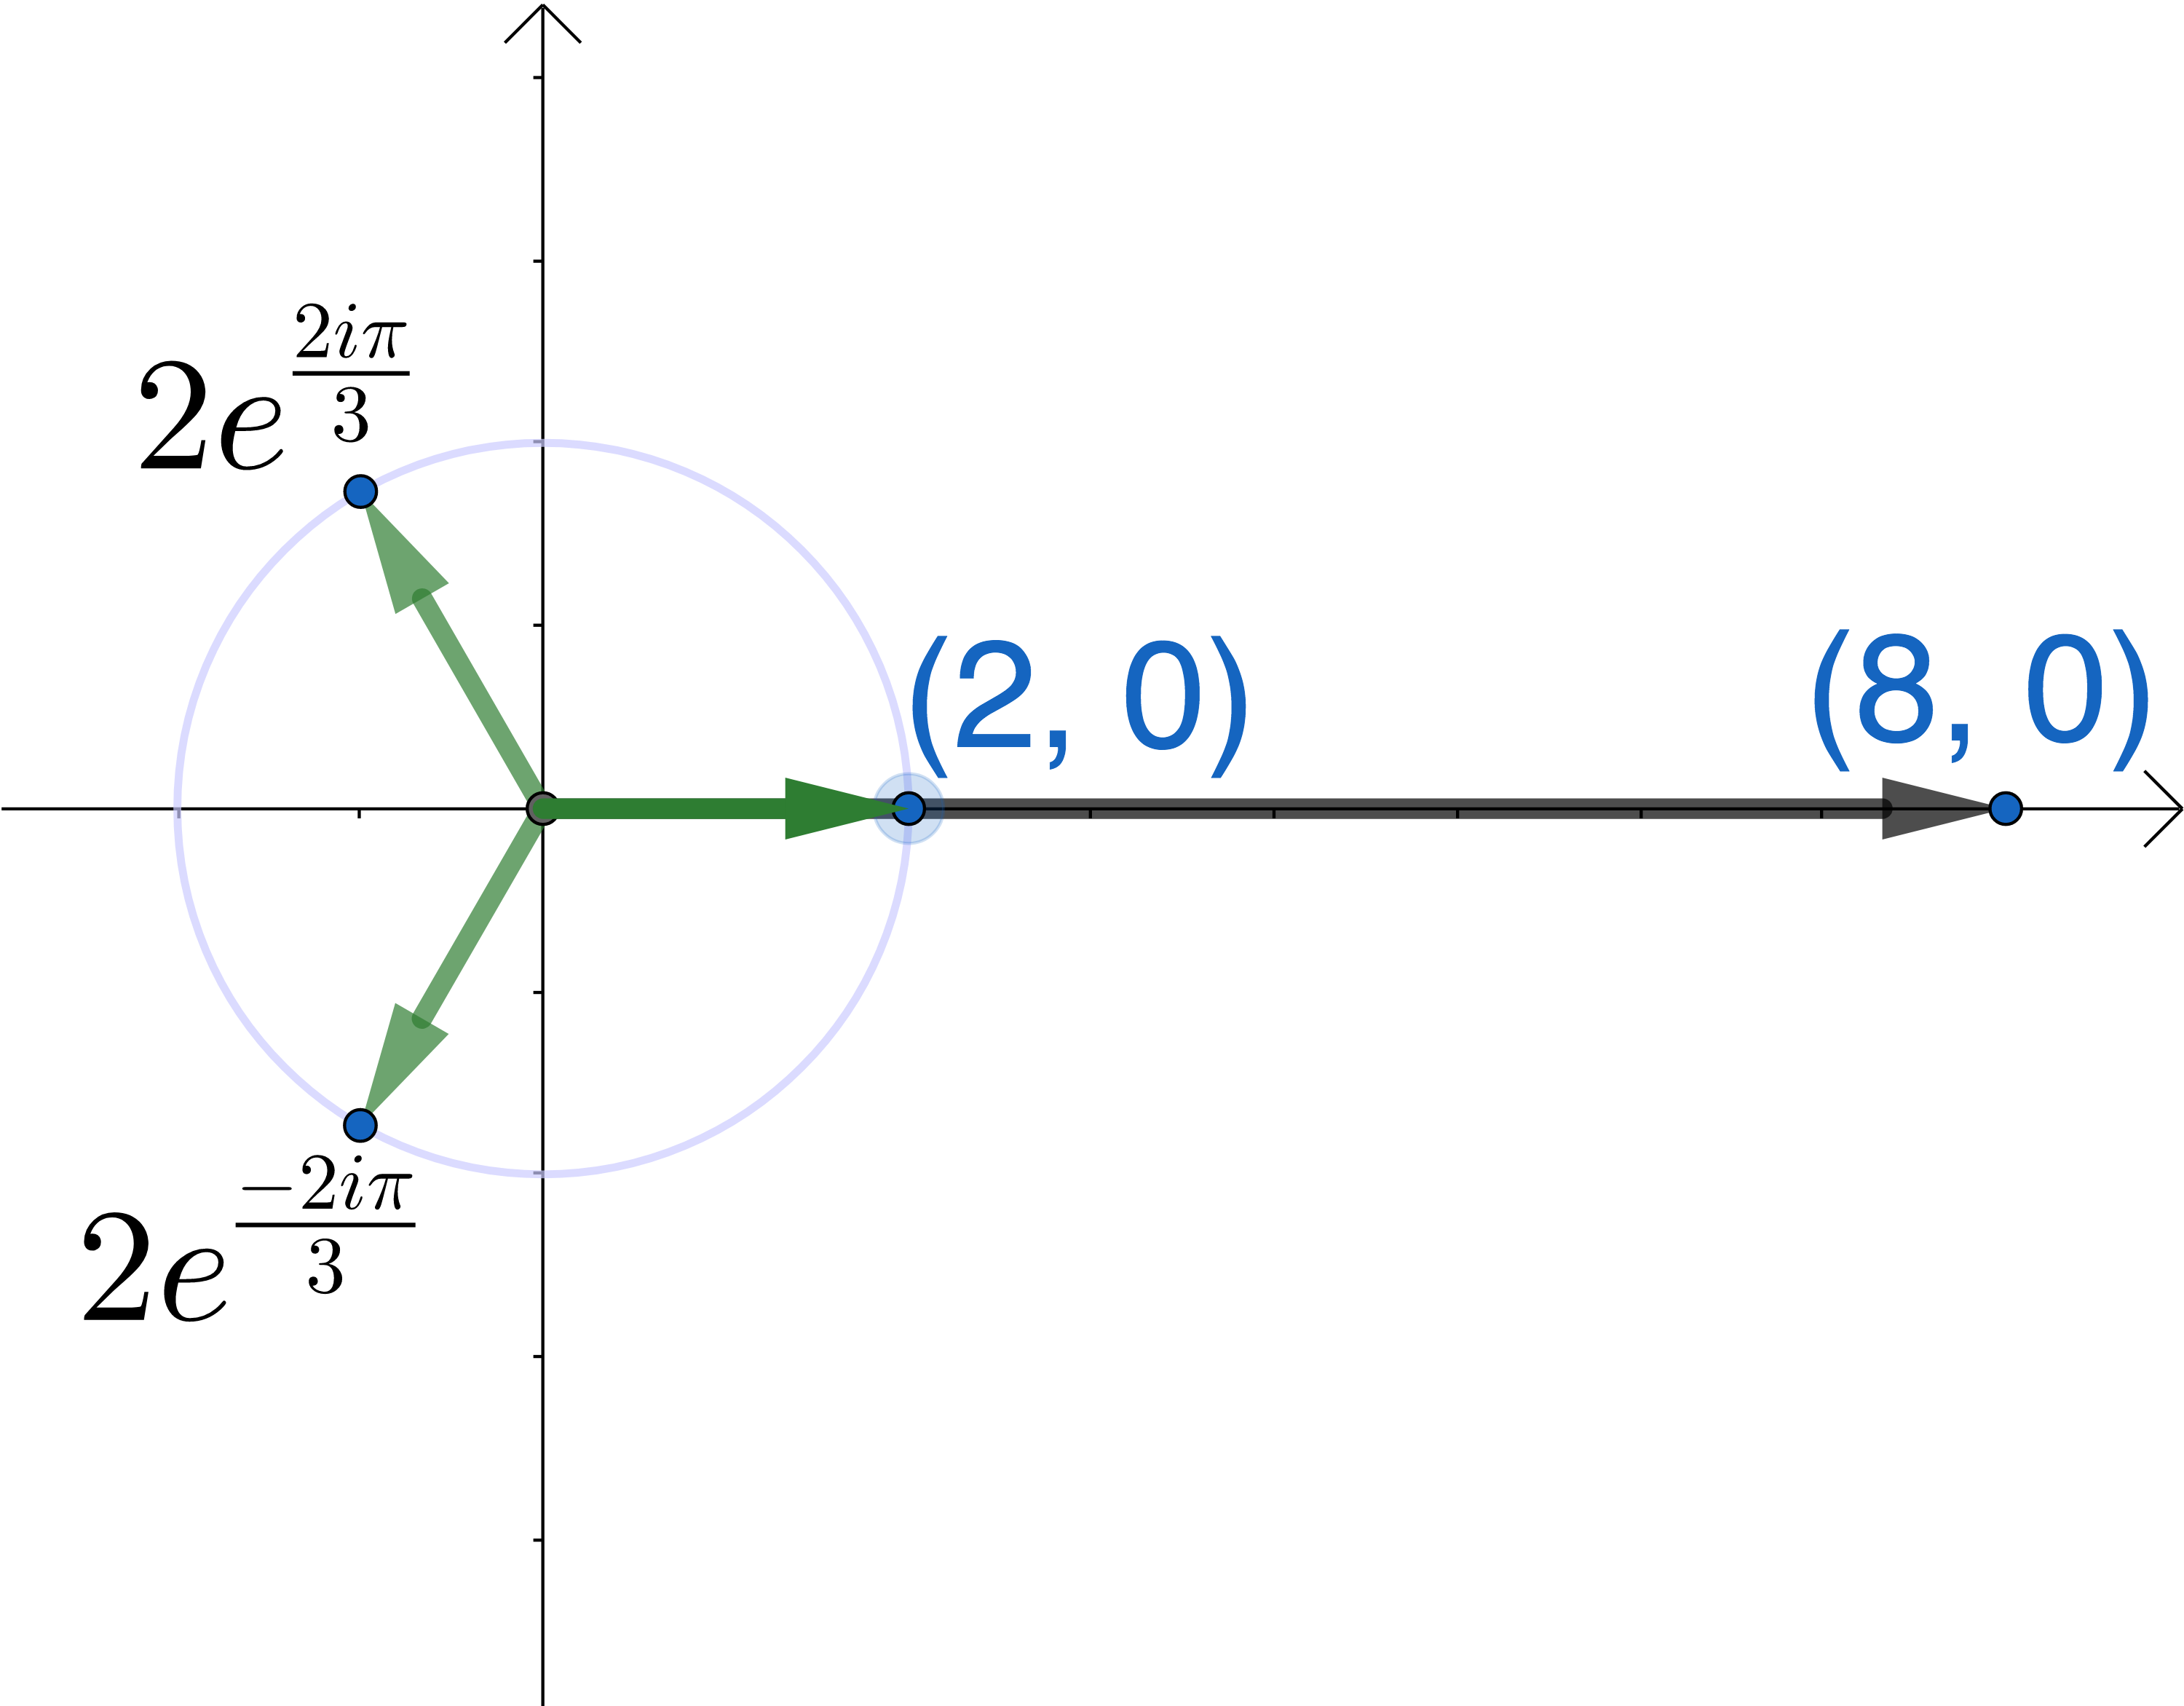
\includegraphics[scale=0.7]{cube-roots-8.png}
\end{center}
\end{frame}

\begin{frame}{Cube roots}
The cube roots of $i$ are $e^{\frac{i\pi}{6}}$, $-i$ and $e^{\frac{5i\pi}{6}}$:
\begin{center}
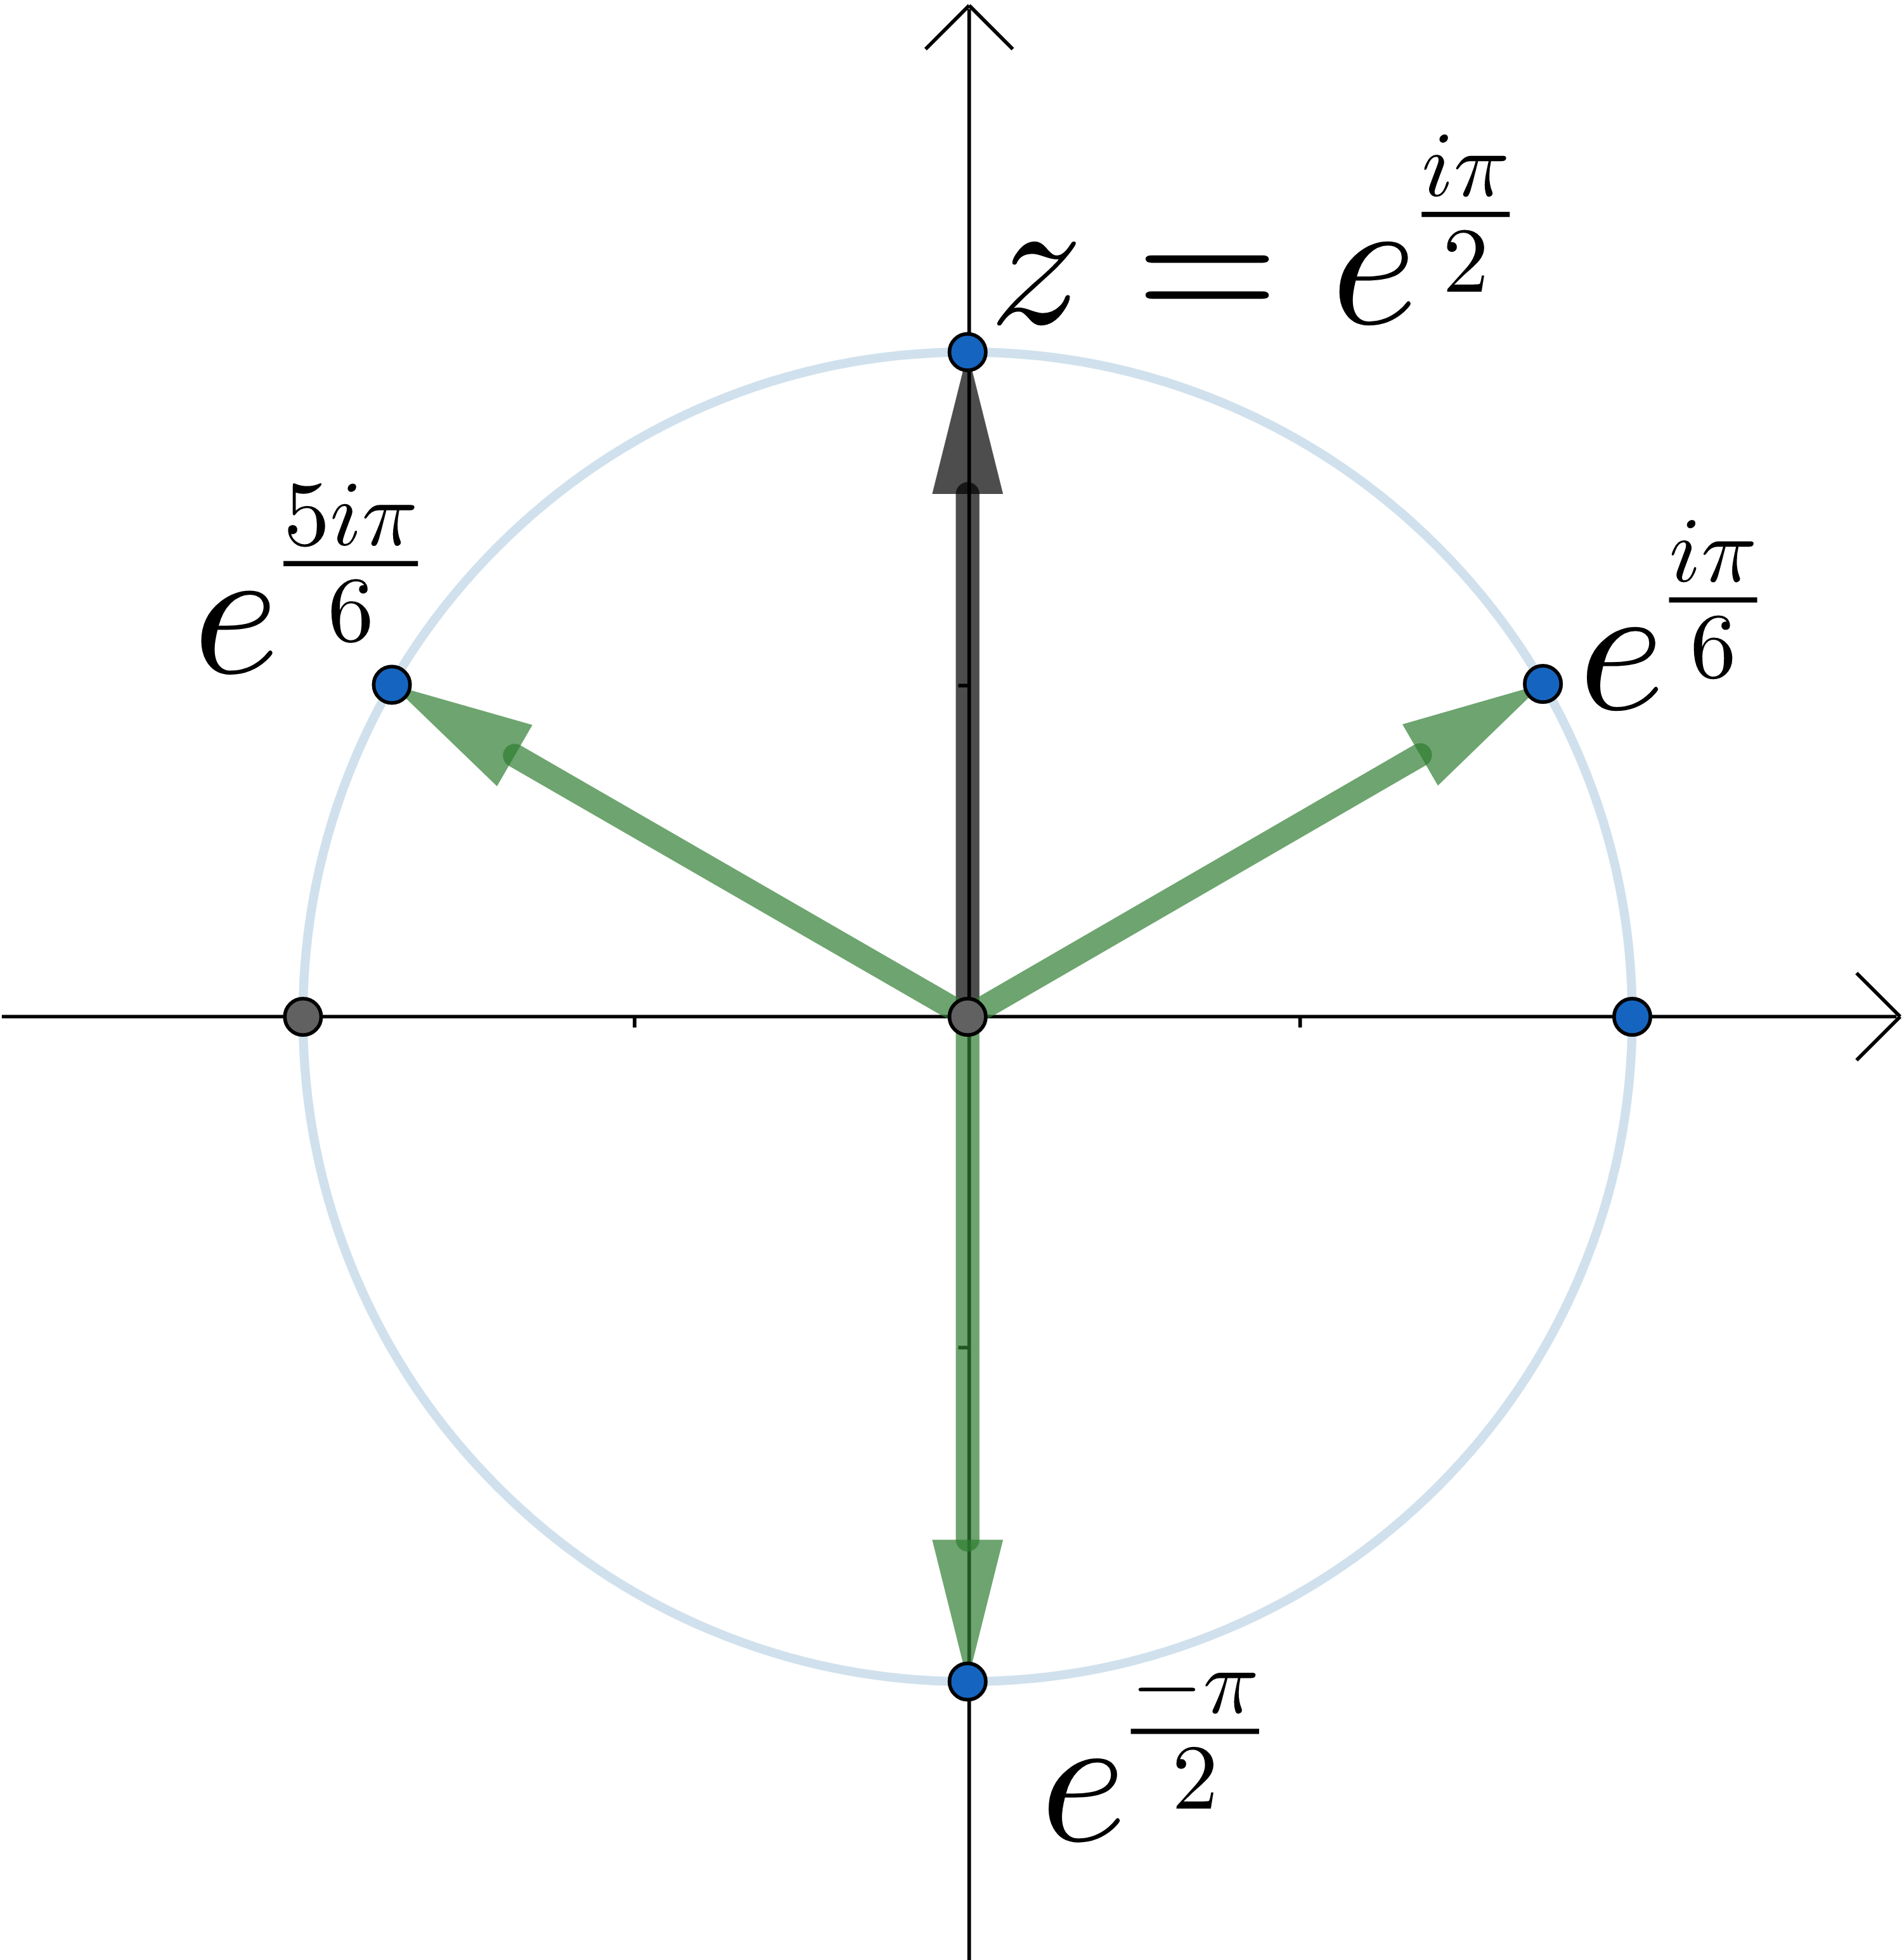
\includegraphics[scale=2]{cube-pi-2.png}
\end{center}
\end{frame}

\begin{frame}{4-th roots}
The fourth roots of unity are: $1$, $i$, $-1$ and $-i$:
\begin{center}
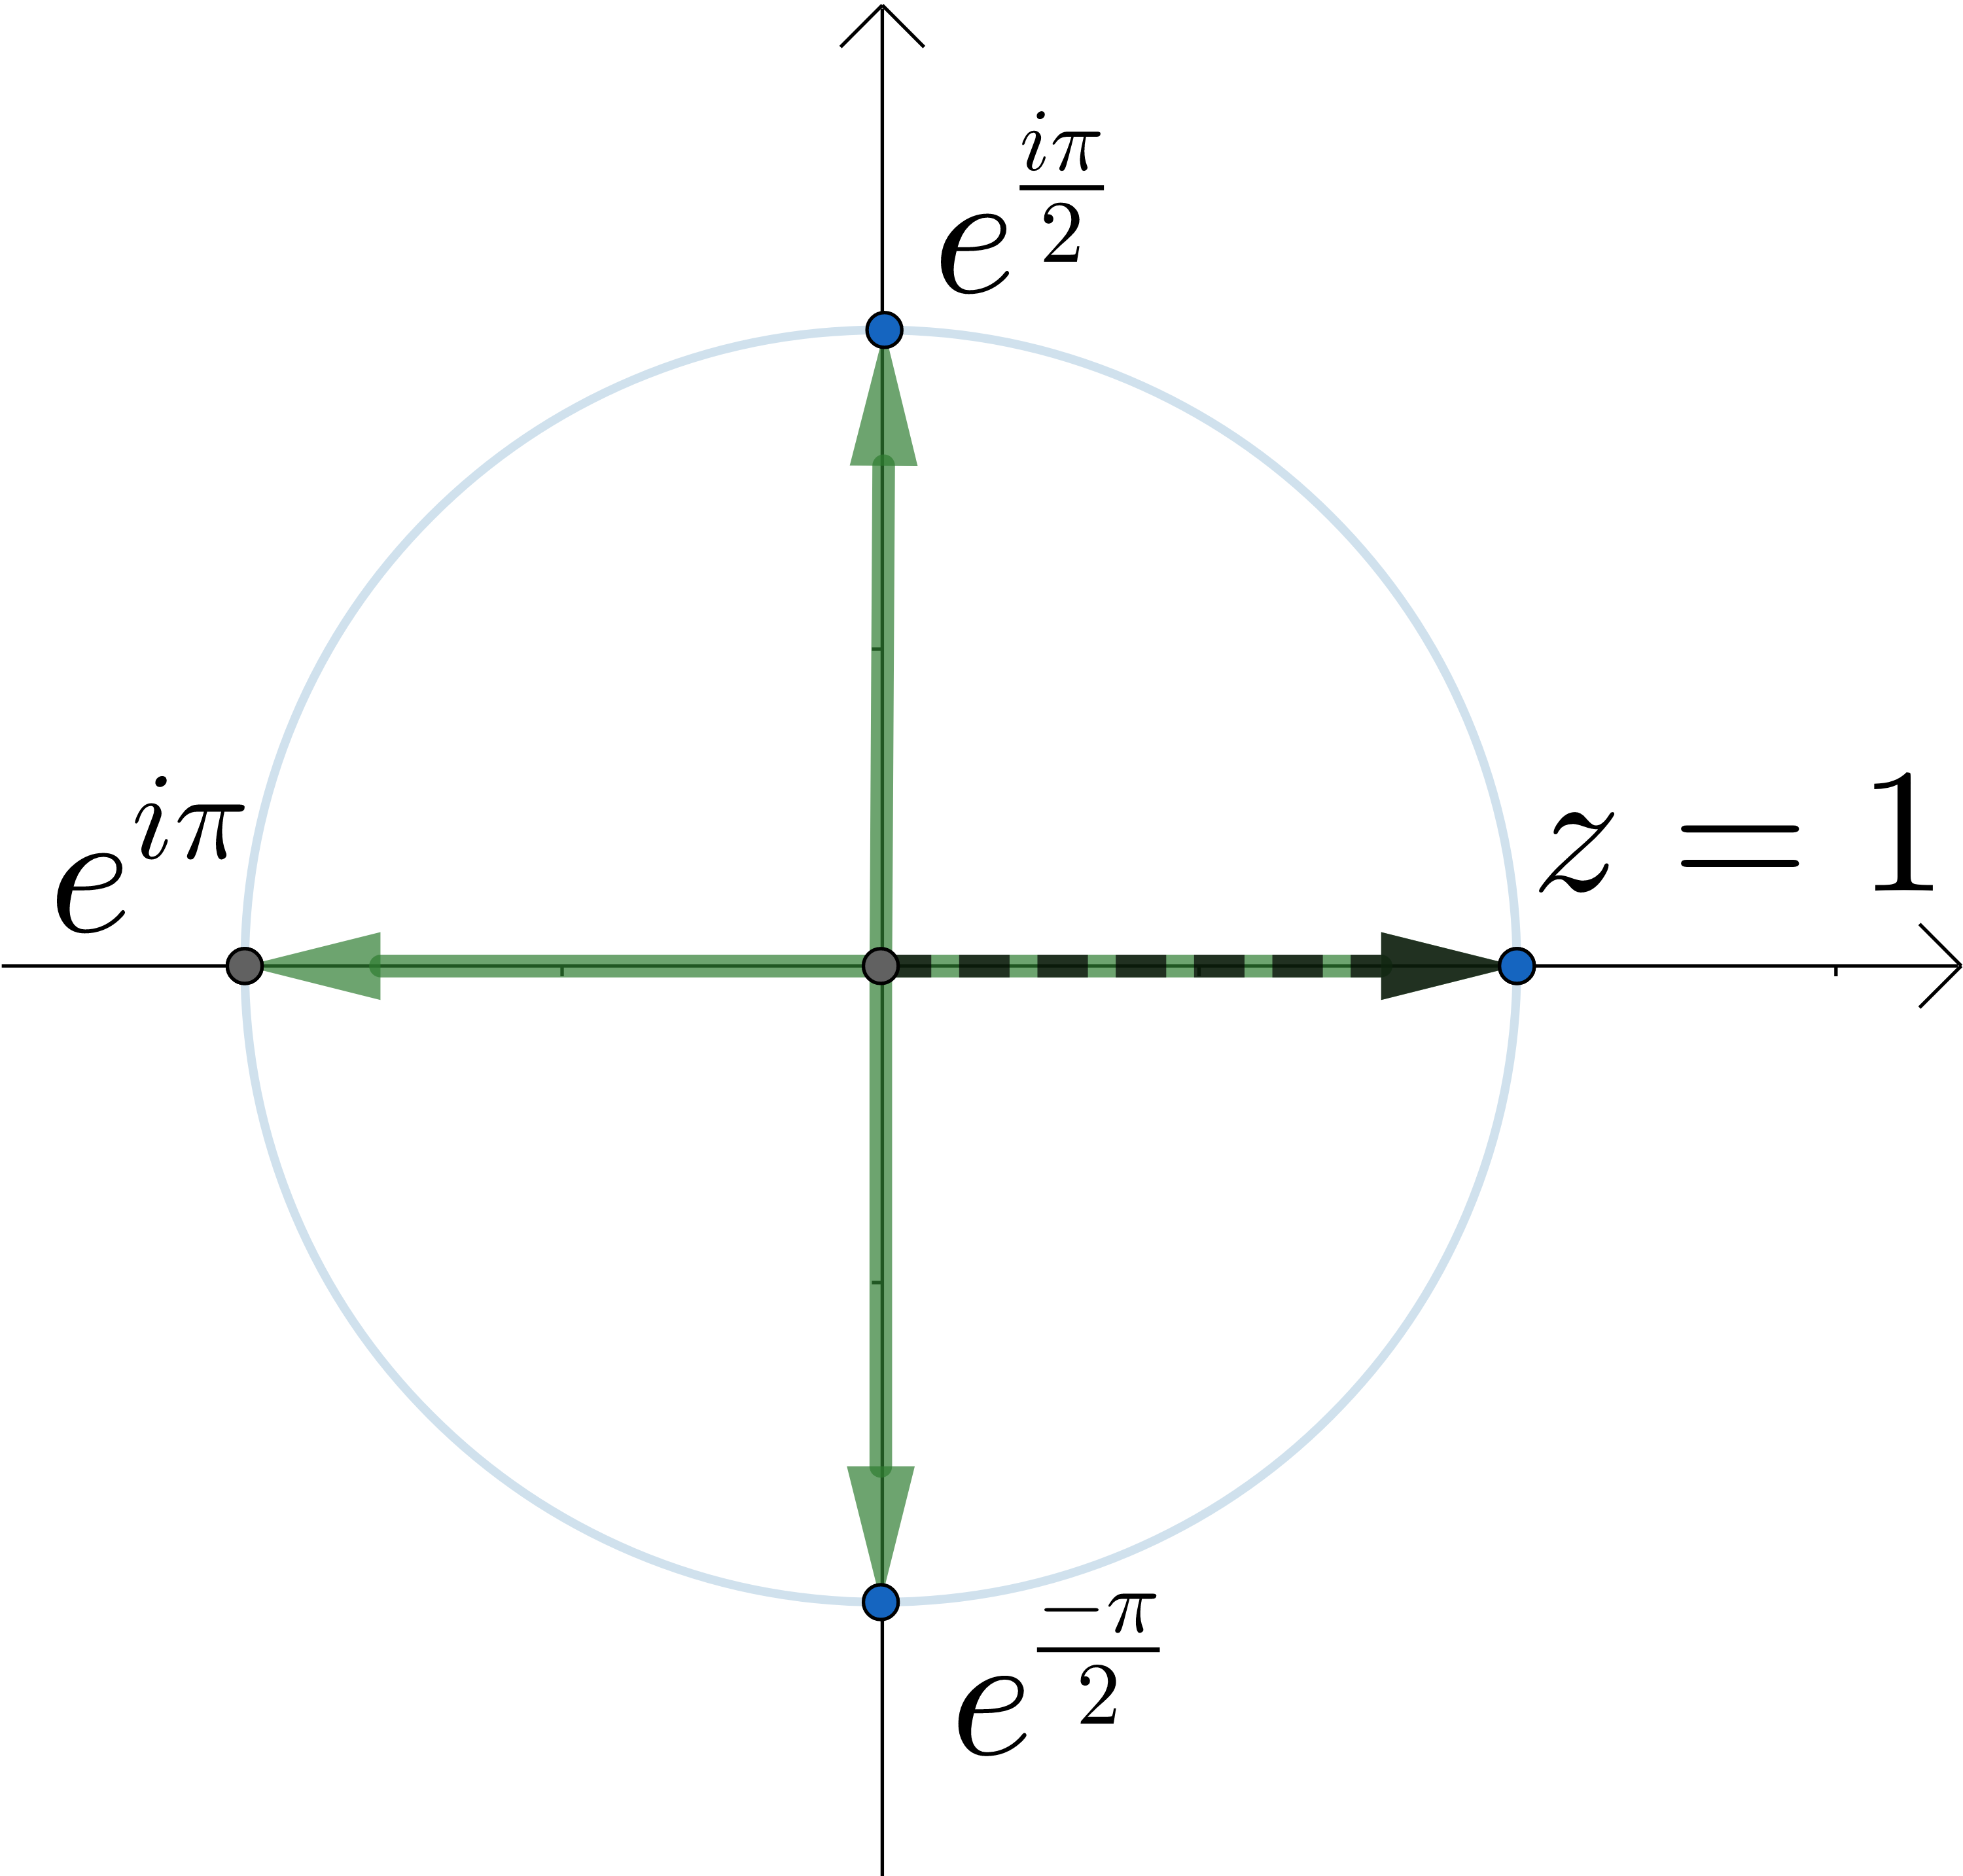
\includegraphics[scale=2]{four-roots-unity.png}
\end{center}
\end{frame}

\begin{frame}{Questions?}
Questions?
\end{frame}

\begin{frame}{Examples}
\begin{example}
Find all solutions to the following equations:
\begin{itemize}
	\item $z^2 = 25$. % ANS: -5 and +5
	\item Find all solutions to $z^2 = -1$ % ANS: i and -i
	\item Find all solutions to $z^2 = e^{\frac{i\pi}{4}}$ % ANS: e^{i*pi/8} and e^{-7*i*pi/8}
	\item Find all solutions to $z^3 = -1$.
	\item Find all solutions to $z^4 = 2(\sqrt{3}i-1)$. % ANS: sqrt{6}/2 + sqrt{2}/2i and + -sqrt{2}/2 +sqrt{6}/2 i and -sqrt{6}/2 - sqrt{2}/2i and  + sqrt{2}/2 -sqrt{6}/2 i
\end{itemize}
\end{example}
\begin{example}
Find all sixth roots of unity.
\end{example}
\end{frame}

\section{Quadratic formula}

\begin{frame}
\begin{beamercolorbox}[sep=12pt,center]{part title}
\usebeamerfont{section title}
\insertsection\par
\end{beamercolorbox}
\end{frame}

\begin{frame}{Quadratic formula}
If $a$, $b$ and $c$ are \emph{complex numbers} then the equation
\begin{equation*}
az^2+bz+c = 0
\end{equation*}
has two solutions given by
\begin{equation*}
	z_1 = \frac{-b+\sqrt{b^2-4ac}}{2a} z_2 = \frac{-b-\sqrt{b^2-4ac}}{2a}
\end{equation*}
\begin{itemize}
	\item We assume $a\neq 0$.
	\item If we use complex numbers we always get two solutions.
\end{itemize}
\end{frame}

\begin{frame}{Galois theory for quadratics}
If $u$ and $v$ are the roots of $f(x) = z^2 + bz+c$ then
\begin{equation*}
(z-u)(z-v) = z^2 - (u+v)z + uv
\end{equation*}
and so
\begin{align*}
b & = -u-v\\
c & = uv
\end{align*}
\begin{itemize}
	\item If $b$ and $c$ are real then either
	\begin{itemize}
		\item $u$ and $v$ are real or
		\item $u = \overline{v}$.
	\end{itemize}
\end{itemize}
\end{frame}

\begin{frame}{Examples}
\begin{example}
Solve $z^2-14z+58 = 0$.
\end{example}
\begin{example}
Find a real quadratic with $5-2i$ as a root. What is the other root?
\end{example}
\begin{example}
Find a real quadratic with $-3+4i$ as a root. What is the other root?
\end{example}
\end{frame}

\begin{frame}
\begin{example}
Find the roots of $z^2-3iz+(-3+i) = 0$.
\end{example}
\begin{example}
Verify that $4-i$ is a root of $z^2 - (2-3i)z-(10+6i) = 0$. Find the other root.
\end{example}
\begin{example}
Solve $z^2-(3-2i)z + (5-i) = 0$.
\end{example}
\end{frame}

\section{Eigenvectors}

\begin{frame}
\begin{beamercolorbox}[sep=12pt,center]{part title}
\usebeamerfont{section title}
\insertsection\par
\end{beamercolorbox}
\end{frame}

\begin{frame}{Simplifying matrix actions}
	If
	\begin{equation*}
		A = \left[\begin{matrix}
			3 & -1\\
			-1 & 3
		\end{matrix}\right]
	\end{equation*}
	then $A$ acts on some vectors in a simplified way:
	\begin{equation*}
		A v_1 = 
		A \left[
		\begin{matrix}
		1\\
		1
		\end{matrix}
		\right] = \left[
		\begin{matrix}
		2\\
		2
		\end{matrix}
		\right] = 2v_1
	\end{equation*}
	and
	\begin{equation*}
	\begin{matrix}
	Av_2 =
	A \left[
	\begin{matrix}
	1\\
	-1
	\end{matrix}
	\right] = 
	\left[
	\begin{matrix}
	4\\
	-4
	\end{matrix}
	\right]
	4v_2
	\end{matrix}
	\end{equation*}
\end{frame}

\begin{frame}{Picture}
\begin{columns}
	\column{0.5\textwidth}
	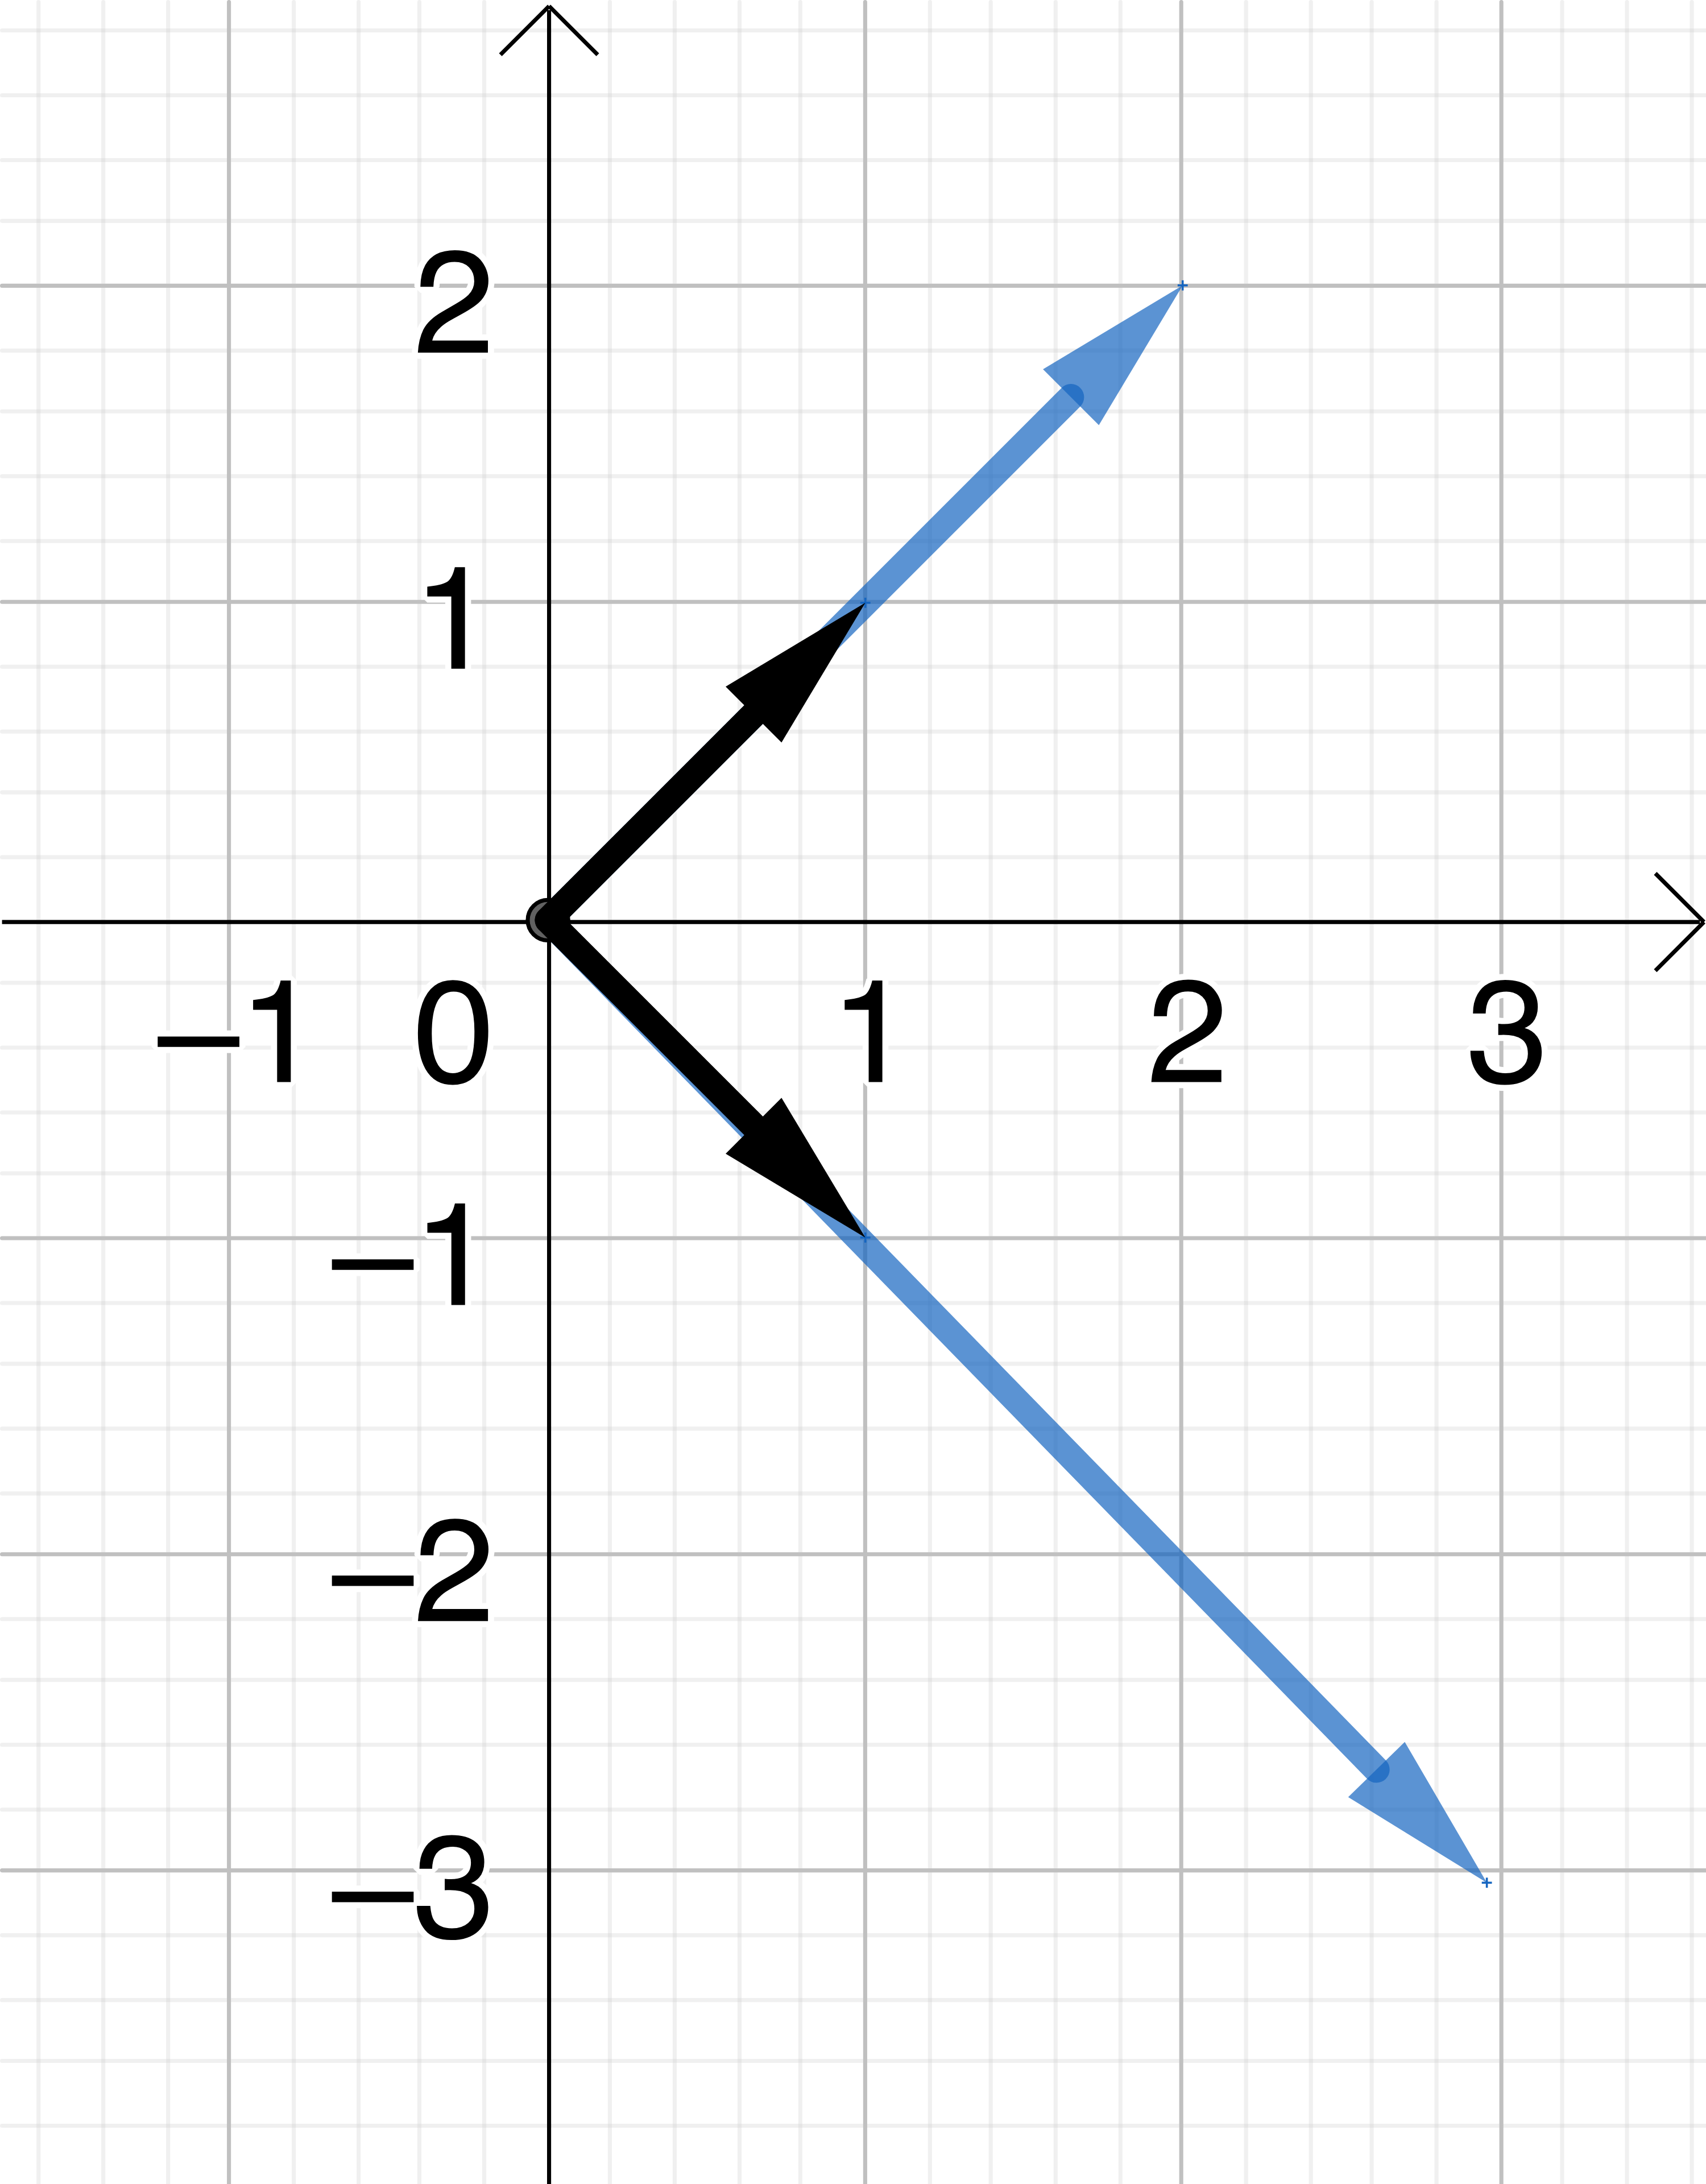
\includegraphics{2d-diag.png}
	\column{0.4\textwidth}
	Since
	\begin{equation*}
		Av_1 = 2v_1
	\end{equation*}
	and
	\begin{equation*}
		Av_2 = 4v_2
	\end{equation*}
\end{columns}
\end{frame}

\begin{frame}{simplifying matrix actions}
	If
	\begin{equation*}
	A = \frac{1}{2}\left[
	\begin{matrix}
	1&1&2\\
	1&1&-1\\
	-1&1&0
	\end{matrix}
	\right]
	\end{equation*}
	then
	\begin{equation*}
		Av_1 = 
		A \left[
		\begin{matrix}
		1\\
		1\\
		0
		\end{matrix}
		\right] = 
		\left[
		\begin{matrix}
		1\\
		1\\
		0
		\end{matrix}
		\right] = v_1
	\end{equation*}
	\begin{equation*}
		Av_2 =
		A \left[
		\begin{matrix}
		-1\\
		1\\
		0
		\end{matrix}
		\right] = \left[
		\begin{matrix}
		0\\
		0\\
		1
		\end{matrix}
		\right] = v_3
	\end{equation*}
	and
	\begin{equation*}
		Av_3 =
		A \left[
		\begin{matrix}
		0\\
		0\\
		1
		\end{matrix}
		\right] =
		\left[
		\begin{matrix}
		1\\
		-1\\
		0
		\end{matrix}
		\right] = -v_2
	\end{equation*}
\end{frame}

\begin{frame}{Picture}
\begin{columns}
	\column{0.7\textwidth}
	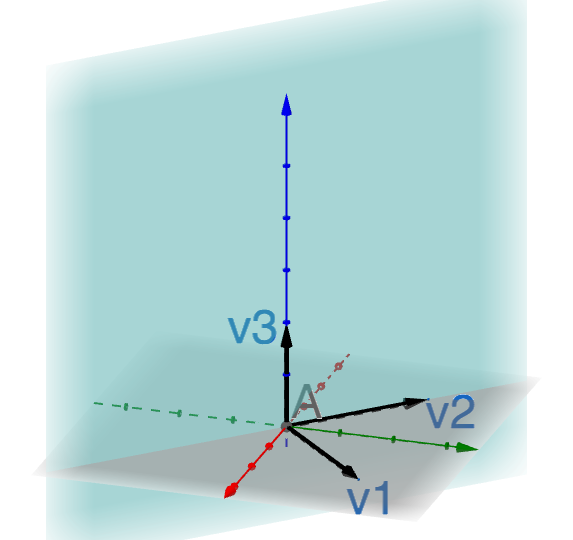
\includegraphics[scale=0.4]{3d-rotation.png}
	\column{0.3\textwidth}
	Blue plane is preserved.
\end{columns}
\end{frame}

\begin{frame}{Eigenvectors and eigenvalues}
\begin{definition}
The matrix $A$ has an \emph{eigenvector $v$ with eigenvalue $\lambda$} iff $v\neq 0$ and 
\begin{equation*}
	Av = \lambda v
\end{equation*}
where $\lambda$ could be any complex number.
\end{definition}
\end{frame}

\begin{frame}{Examples}
\begin{example}
$\left[
\begin{matrix}
3&0\\
0&5
\end{matrix}
\right]$ has eigenvectors $\left[
\begin{matrix}
1\\
0
\end{matrix}
\right]$ and $\left[
\begin{matrix}
0\\
1
\end{matrix}
\right]$ with eigenvalues $3$ and $5$ respectively.
\end{example}
\begin{example}
$\left[
\begin{matrix}
3&-1\\
-1&3
\end{matrix}
\right]$ has eigenvectors $\left[
\begin{matrix}
1\\
1
\end{matrix}
\right]$ and $\left[
\begin{matrix}
1\\
-1
\end{matrix}
\right]$ with eigenvalues $2$ and $4$ respectively.
\end{example}
\end{frame}

\begin{frame}{Finding eigenvalues}
Since
\begin{equation*}
Av = \lambda v \iff (A-\lambda I)v = 0
\end{equation*}
and $v\neq 0$ we need to find all $\lambda$ such that 
\begin{equation*}
	A-\lambda I
\end{equation*}
is \emph{not} invertible.\vfill
\begin{definition}[Characteristic polynomial]
	The \emph{characteristic polynomial of a matrix $A$} is
	\begin{equation*}
	 	\chi_A(\lambda) = det(A-\lambda I)
	 \end{equation*} 
\end{definition}
So to find the eigenvalues we find the roots of the characteristic polynomial.
\end{frame}

\begin{frame}{Examples}
\begin{example}
	Find the eigenvalues of
	\begin{equation*}
		\left[
		\begin{matrix}
		4&-2\\
		-1&3
		\end{matrix}
		\right]
	\end{equation*}
\end{example}
\begin{example}
	Find the eigenvalues of
	\begin{equation*}
		\left[
		\begin{matrix}
		4&1&2\\
		0&3&-2\\
		0&-1&2
		\end{matrix}
		\right]
	\end{equation*}
\end{example}
\end{frame}

\end{document}